\chapter{序論}
\section{背景}
\begin{figure}[ht]
    \centering
    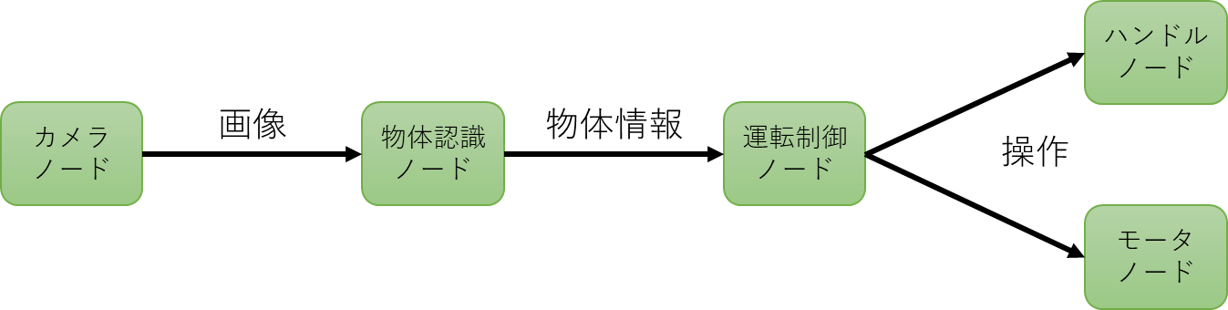
\includegraphics[width=15cm]{images/fig1_rosprograming_configuration.png}
    \caption{ROSプログラミングモデルの例}
    \label{fig:ros_programing_model}
\end{figure}
さまざまな産業向けやエンターテイメント関連のロボットシステム,自動車の自動運転技術やIoTシステムのソフトウェア開発をサポートするフレームワークとしてRobot Operating System(以下,ROS)の普及が進んでいる[1].
ROSのプログラミングモデルは,システムの各機能を独立したプログラムモジュール(ノード)として設計することにより,汎用性と再利用性を向上させて,各機能モジュール間のデータ交換を規定することで,効率的かつ柔軟なシステム構築を可能にしている.
例として図1.1に示す.
カメラを操作して周囲の環境を撮影するノード,画像からオブジェクトを識別するノード,オブジェクトのデータをもとに動作制御を実行するノードを連携させることで,自動運転車の基本機能の一部を容易に実装できる.
\\ ROSのプログラミングモデルは,ロボット/IoTとクラウドが協力する分散型システムにおいても有効である.
ロボットシステムのソフトウェア処理は,外界の情報を取得する「センサー」,取得した情報を処理する「知能・制御系」,実際に動作するモーターなどの「動力系」の3要素に分類できる[2].
クラウドとロボットが連携して高度なロボットシステムを実現するクラウドロボティクス[3]において,主に知能・制御系のノードを高い計算能力を持つクラウドに優先して配置することで,高度な知能・制御処理の実現を促進できる.
さらに,ロボットが取得した情報や状態などをクラウドに集約・保存することで,複数のロボット間での情報共有と利用を容易にする.
\section{課題}
一方で,現行のROS実装では,各ノードの配置をシステム起動時に静的に設定する必要があり,クラウドとロボット間の最適なノード配置を事前に設計する必要がある.
実際の環境で動作するロボットは,ネットワークの状況やバッテリー残量の変動など,システム運用前に予測することが困難な状況変化に対応する必要があり,設定したクラウドとロボット間のノード配置が最適でなくなる可能性がある.
このような状況変化への対応として,ノードを動的に再配置するライブマイグレーション技術があるが,多くの場合でクラウドとロボット間のCPUアーキテクチャが異なり,命令セットがそれぞれ違うため,実行中のノードをシステム運用中にマイグレーションすることは技術的に困難である.
\section{目的}
菅ら[4]は,WebAssembly(以下,Wasm)を用いることで,クラウドとロボット間での実行状態を含む稼働中ノードの動的にマイグレーションする手法を実現した.
WasmとはWeb上で高速にプログラムを実行するために設計された仮想命令セットアーキテクチャのことで,1つのバイナリが複数のアーキテクチャで動作するため,異なるCPUアーキティクチャ間でのマイグレーションに適しているといえる.
課題として,ROSをWasm化したことでライブマイグレーション後のファイルサイズのオーバーヘッドが増大し,ノードの実行時間が大幅に増えてしまう問題が残った.
柿本ら[5]は,組込みデバイス向けの軽量なROSランタイム実装であるmROS 2-POSIXを採用し,ROSランタイムのWasm化にともなうオーバヘッド増加に対処した.
しかし,mROS 2-POSIXはネットワークスループットのマイクロベンチマークに留まっている[6].
また,柿本らによって実現したmROS 2-POSIXをWasm化したmROS 2-Wasmも実際のアプリケーションでは評価されていない[5].
そのため,ライブマイグレーション後のオーバーヘッド増加を解決するロボットソフトウェア基盤として,アプリケーションが複雑化した場合の動作が明らかでない.
\\ 本研究では,ノードの動的マイグレーションに向けたmROS 2-POSIXとmROS 2-Wasmの性能評価を行い,ネイティブROSと比べて動的配置機構実現後のロボットソフトウェア基盤として優位性を明らかにすることを目指している.
アプローチとして,動的配置機構を実現するのに適したアプリケーションをmROS 2-POSIX,mROS 2-Wasm,ネイティブROSで実装し,通信時間とメモリ消費量を比較評価する.
ネイティブROSにはラズパイマウス[22]と呼ばれる2つの車輪を回転することで動作するロボットのライントレース実装があり,本実装として,mROS 2-POSIXとmROS 2-Wasmにそのアプリケーションを移植する.
このライントレースノードは,組込みデバイス上で動作し,主な機能はPub/Sub通信を使用しているため,本研究の実装するアプリケーションとして適しているうちの一つである.このライントレースノードの実装により,mROS 2-POSIXとmROS 2-Wasmのロボットソフトウェア基盤としての拡張性を示すことができ,評価によって,実アプリケーション上でmROS 2-POSIXとmROS 2-Wasmの軽量性を示す.
\section{章構成}
本評価では,ライントレースノードを各環境で動作させ,いくつかのトピックに対して,Pub/Sub通信のにかかる時間を通信性能とし,計測を行った.
また,各環境でRSS(Resident Set Size 物理消費メモリ)を測定するために実行時のプロセスIDを取得し,そのプロセスに割り当てられているRSSを計測した.
この結果を実験結果として本論文に示す.
\\ 本論文は,全7章から構成されている.第1章は,本研究における背景と課題,目的について述べた.第2章は,ROSやmROS 2-POSIX,WebAssemblyについて述べる.第3章では,Wasm仮想マシンを用いたmROS 2-POSIX環境であるmROS 2-Wasmに関する先行研究について述べる.第4章では,本研究のライントレースノードを各環境の実装について説明する.第5章では,実験結果を示し,結果から得られた知見から考察を述べる.第6章では,関連研究について述べる.第7章では,本研究のまとめと今後の課題について述べる.
%%本研究の部分が悪い.全部評価に集約してるから前振りがなんなのか並べて本研究で回収する